\section[Decision Trees for Classification]{Decision Trees for Classification}

\subsection[CART Algorithm]{CART Algorithm}

\begin{frame}{One-Dimensional and Linearly Separable Problem}
	\begin{figure}
		\centering
		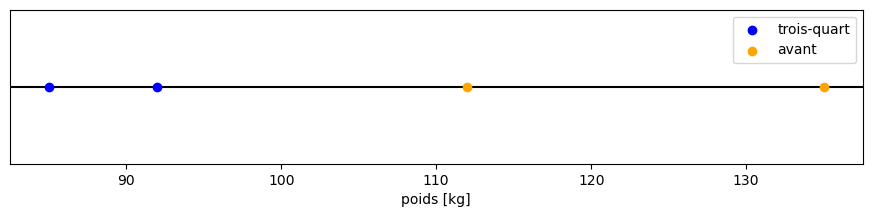
\includegraphics[width=0.85\linewidth]{Images/lineairement_separable_1}
		\label{fig:lineairement_separable_1}
	\end{figure}				
	In the example above, we seek to classify rugby players based on their weight. This problem is linearly separable: there is at least one weight threshold that allows us to \textbf{perfectly} separate the forwards from the backs.
	
	\vfill
	\pause
	The core idea consists of choosing a weight threshold that splits the data into two groups such that the weighted sum of the groups' \textbf{entropies} is \textbf{minimized}.
	
	\vfill
	\pause
	This is the operational principle of the \textbf{CART} algorithm: Classification And Regression Trees.
\end{frame}

\begin{frame}{One-Dimensional and Linearly Separable Problem}
	For a given splitting weight threshold, the entropy is calculated as:
	\begin{align*}
		H(P) &= P(X = \text{"Back"}) I(X = \text{"Back"}) \\
		&\quad + P(X = \text{"Forward"}) I(X = \text{"Forward"}) \\
		&= - P(X = \text{"Back"}) \log P(X = \text{"Back"}) \\
		&\quad - P(X = \text{"Forward"}) \log P(X = \text{"Forward"})
	\end{align*}
	Consider the following split options:
	\begin{itemize}
		\item Split weight: 90 kilograms
		\begin{itemize}
			\item In the left group: 1 back. $H_{\text{left}} \to 0$.
			\item In the right group: 1 back and 2 forwards: $H_{\text{right}} = - \frac{1}{3} \log \frac{1}{3} - \frac{2}{3} \log \frac{2}{3} \approx 0.64$
		\end{itemize}
		\pause
		\item Split weight: 100 kilograms
		\begin{itemize}
			\item In the left group: 2 backs. $H_{\text{left}} \to 0$.
			\item In the right group: 2 forwards: $H_{\text{right}} \to 0$.
		\end{itemize}		
	\end{itemize}
	\pause
	We therefore select a split weight threshold of 100 kilograms since the sum of the group entropies is zero.
\end{frame}

\begin{frame}{Algorithm for a One-Dimensional Problem}
	Given training data $X \in \mathcal{X}$ with $\mathcal{X} \subset \R$ and $Y \in\{0, 1\}$:
	\begin{enumerate}
		\item We sort the training data $\mathcal{D} = \{(x^{(i)}, y^{(i)})\}_{i=1}^n$ by increasing value of $x$.
		\pause
		\item For each $k \in \llbracket 2; n \rrbracket$, we evaluate a split value $x^* = \left(x_{(k)} + x_{(k - 1)}\right) / 2$ where $x_{(k)}$ represents the $x$ observation at rank $k$. $x^*2$ is the midpoint.
		\begin{itemize}
			\item We compute the entropy in the left group (\textbf{branch}): $\{(x, y) \in \mathcal{D} \mid x < x^*\}$.
			\item We compute the entropy in the right group (\textbf{branch}): $\{(x, y) \in \mathcal{D} \mid x > x^*\}$.
			\item We compute the sum of the two entropies, weighted by the number of observations in each group.
		\end{itemize}
		\pause
		\item We select the value of $x^*$ that minimizes this weighted sum.
	\end{enumerate}
\end{frame}

\begin{frame}{Algorithm for a Multi-Dimensional Problem}
	Given training data $X \in \mathcal{X}$ with $\mathcal{X} \subset \R^d$ and $Y \in\{0, 1\}$:
	\begin{enumerate}
		\item For each $j \in \llbracket 1; d \rrbracket$, we apply the one-dimensional problem algorithm considering only feature $X_j$.
		\begin{itemize}
			\item We thus obtain a weighted sum for each value of $j$.
			\item Each weighted sum is associated with an optimal split value $x_j^*$.
		\end{itemize}
		\pause
		\item We select the feature index $j$ for which the weighted sum of entropies is minimized, along with its associated split value $x_j^*$.
		\pause
		\item We split the observations into two groups:
		\begin{itemize}
			\item Left: $\{(x, y) \in \mathcal{D} \mid x_j < x_j^*\}$.
			\item Right: $\{(x, y) \in \mathcal{D} \mid x_j > x_j^*\}$.
		\end{itemize}
		\pause
		\item We assign a depth of 1 to each resulting group.
	\end{enumerate}
\end{frame}

\begin{frame}{Recursive Algorithm}
	The algorithm is recursive. We therefore re-apply the multi-dimensional problem algorithm to each group created this way.
	\begin{enumerate}
		\item For each previously created group, we check for a stopping criterion:
		\begin{itemize}
			\item If the depth of the group reaches a fixed maximum value, we stop. Depth represents the number of recursive splits from the initial data (the maximum number of \textbf{branches}).
			\item If the entropy of the group reaches a fixed minimum value, we stop.
			\item If the group size reaches a fixed minimum number of observations, we stop.
		\end{itemize}
		\item If a stopping criterion is met, we associate with this group the proportion of observations for which $Y = 1$. This value will allow us to make predictions later.
		\item If no stopping criterion is encountered, we split the parent group into two new child groups following the multi-dimensional algorithm.
		\item We assign to each of these child groups the depth of the parent group plus 1.
	\end{enumerate}
\end{frame}

\begin{frame}{Decision Making}
	In a decision tree, groups are commonly referred to as \textbf{leaves}. Figuratively, a tree splits data into \textbf{branches}. When a stopping criterion is met, splitting stops within that branch, which then becomes a leaf.
	
	\vfill
	\pause
	
	Once all groups have been identified by the recursive algorithm, to perform a prediction on inference data $x_i$:
	\begin{enumerate}
		\item We determine the group (leaf) in which the inference point $x_i$ falls.
		\pause
		\item We return the proportion of observations $Y = 1$ stored within this group: this represents the probability prediction of the algorithm.
	\end{enumerate}
\end{frame}

\subsection[Visualization]{Visualization}

\begin{frame}{Rugby Players Example}
	\begin{columns}
		\begin{column}{0.5\textwidth}
			\begin{figure}
				\centering
				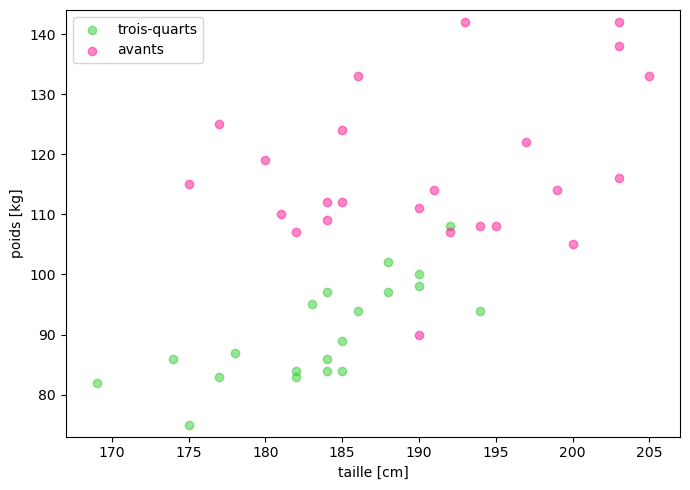
\includegraphics[width=1.0\linewidth]{Images/exemple_rugby_1}
				\label{fig:exemple_rugby_1}
			\end{figure}			
		\end{column}
		\begin{column}{0.5\textwidth}
			In the adjacent plot:
			\begin{itemize}
				\item We observe that forwards are generally both taller and heavier.
				\item With a few exceptions, we could almost have a linearly separable problem.
			\end{itemize}
		\end{column}
	\end{columns}	
\end{frame}

\begin{frame}{Rugby Players Example}
	\begin{columns}
		\begin{column}{0.6\textwidth}
			\begin{figure}
				\centering
				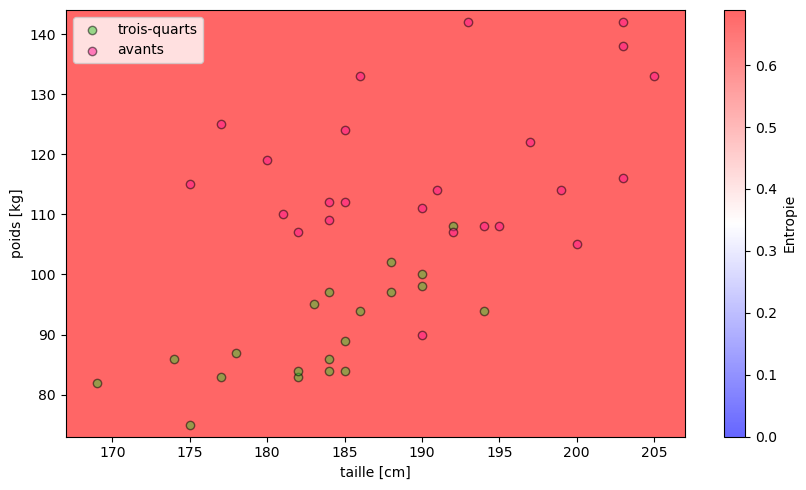
\includegraphics[width=1.0\linewidth]{Images/exemple_rugby_2}
				\label{fig:exemple_rugby_2}
			\end{figure}			
		\end{column}
		\begin{column}{0.4\textwidth}
			This represents the initial entropy of our dataset before the decision tree begins to \textbf{split} the regions.
		\end{column}
	\end{columns}	
\end{frame}

\begin{frame}{Rugby Players Example}
	\begin{columns}
		\begin{column}{0.6\textwidth}
			\begin{figure}
				\centering
				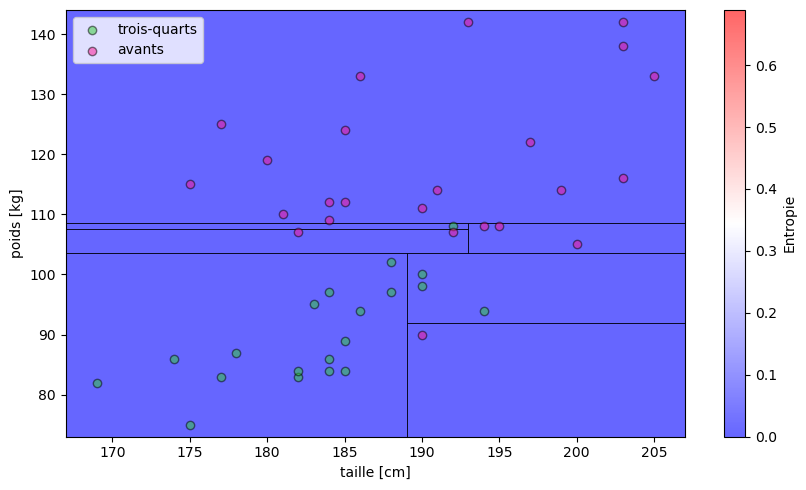
\includegraphics[width=1.0\linewidth]{Images/exemple_rugby_3}
				\label{fig:exemple_rugby_3}
			\end{figure}			
		\end{column}
		\begin{column}{0.4\textwidth}
			After the splits performed by the tree, we now see that each region has zero entropy. This is because each region contains either exclusively forwards or exclusively backs.
		\end{column}
	\end{columns}	
\end{frame}

\begin{frame}{Rugby Players Example}
	\begin{columns}
		\begin{column}{0.6\textwidth}
			\begin{figure}
				\centering
				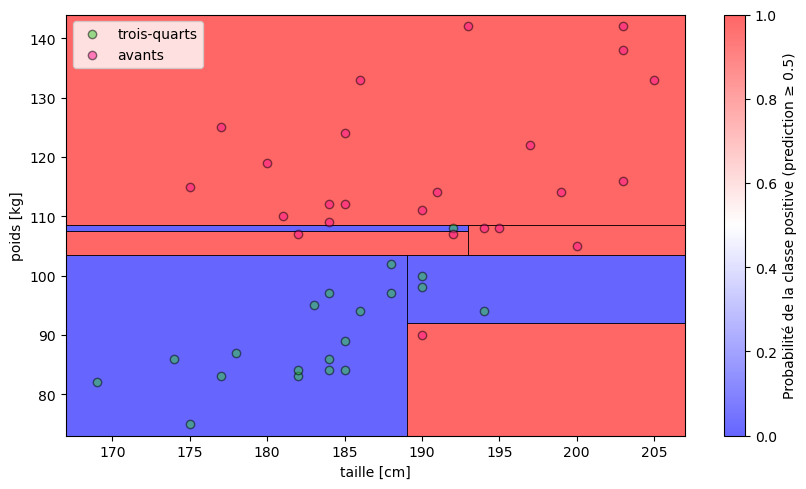
\includegraphics[width=1.0\linewidth]{Images/exemple_rugby_4}
				\label{fig:exemple_rugby_4}
			\end{figure}			
		\end{column}
		\begin{column}{0.4\textwidth}
			This represents the tree's final decision boundary (assuming a decision threshold $\theta = 0.5$). Since each region has zero entropy, the prediction yields a probability of either 0 or 1.
		\end{column}
	\end{columns}	
\end{frame}

\begin{frame}{A Second Example}
	In this second example, we observe how split zones that exhibit low entropy are associated with regions where probabilities are highly distinct (0 or 1). Conversely, regions retaining high entropy are associated with intermediate probabilities.
	\begin{columns}
		\begin{column}{0.5\textwidth}
			\begin{figure}
				\centering
				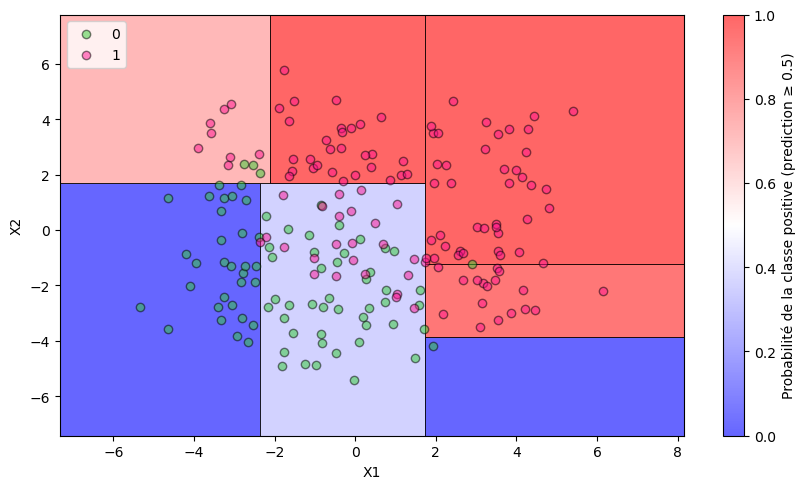
\includegraphics[width=1.0\linewidth]{Images/exemple_jouet_1}
				\label{fig:exemple_jouet_1}
			\end{figure}			
		\end{column}
		\begin{column}{0.5\textwidth}
			\begin{figure}
				\centering
				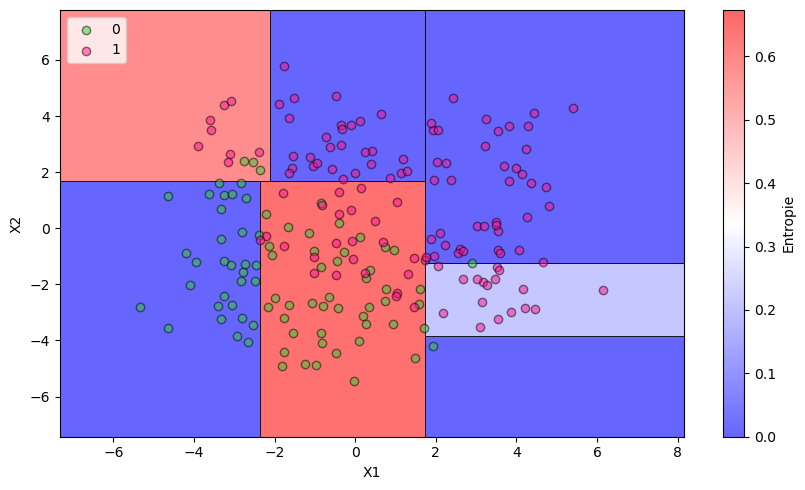
\includegraphics[width=1.0\linewidth]{Images/exemple_jouet_2}
				\label{fig:exemple_jouet_2}
			\end{figure}			
		\end{column}
	\end{columns}	
\end{frame}

\begin{frame}{A Second Example}
	We can adjust the stopping criteria (depth, minimum size, minimum entropy) to obtain a \textit{perfect} fit on the training data:
	\begin{columns}
		\begin{column}{0.5\textwidth}
			\begin{figure}
				\centering
				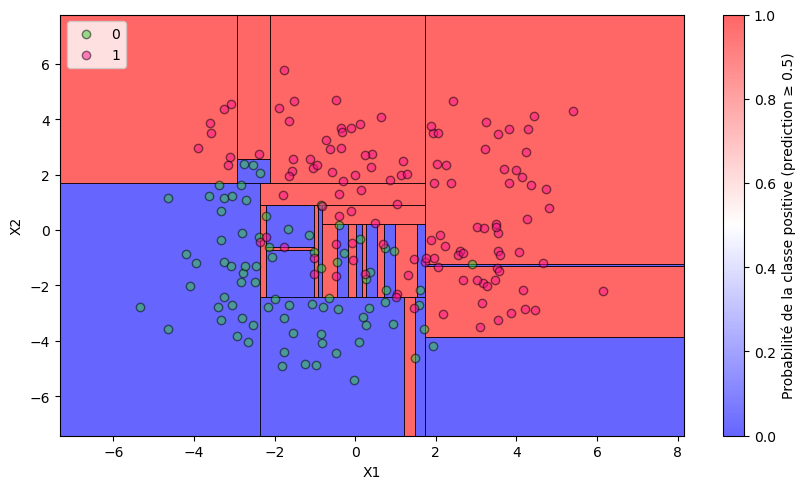
\includegraphics[width=1.0\linewidth]{Images/exemple_jouet_3}
				\label{fig:exemple_jouet_3}
			\end{figure}			
		\end{column}
		\begin{column}{0.5\textwidth}
			\begin{figure}
				\centering
				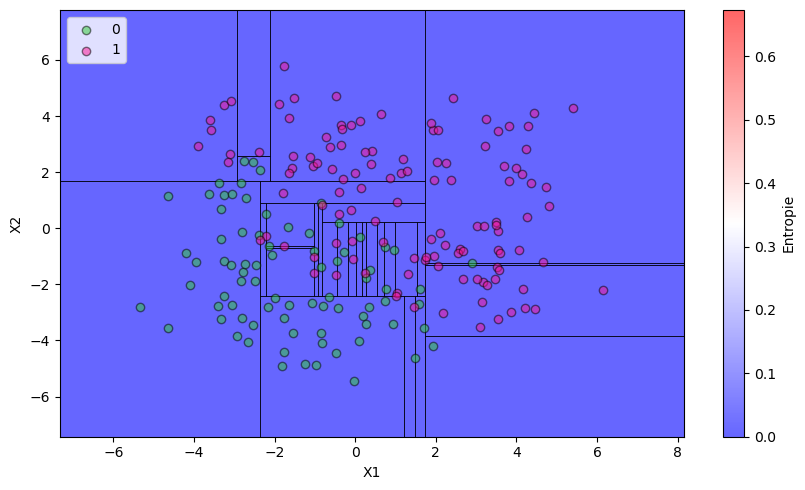
\includegraphics[width=1.0\linewidth]{Images/exemple_jouet_4}
				\label{fig:exemple_jouet_4}
			\end{figure}			
		\end{column}
	\end{columns}	
\end{frame}

\begin{frame}{Bias / Variance Trade-off}
	\begin{itemize}
		\item A \textit{perfect} split on the training data does not guarantee a \textit{perfect} split on the test data.
		\pause
		\item Tuning the stopping criteria too aggressively can lead the algorithm to \textbf{overfitting}.
		\pause
		\item In a decision tree, the trade-off between bias (underfitting) and variance (overfitting) is managed using the stopping criteria:
		\begin{itemize}
			\item \textbf{Minimum leaf size}: a high value introduces bias, while a low value increases variance.
			\item \textbf{Minimum entropy}: a high value introduces bias, while a low value increases variance.
			\item \textbf{Maximum depth}: a low value introduces bias, while a high value increases variance.
		\end{itemize}
	\end{itemize}
\end{frame}